% Ubah kalimat sesuai dengan judul dari bab ini
\chapter{PROFIL PERUSAHAAN}

% Ubah konten-konten berikut sesuai dengan yang ingin diisi pada bab ini

\section{Sejarah PT. NASA}

PT. NASA berdiri pada \lipsum[11]

\lipsum[12][1-10]

\section{Visi dan Misi}

PT. NASA memiliki \lipsum[13][1-3] sebagai berikut:

\begin{enumerate}[nolistsep]

  \item \textbf{Visi PT. NASA}

  Menjadi \lipsum[13][4-7]

  \item \textbf{Misi PT. NASA}

  \begin{enumerate}[nolistsep]

    \item Membuat \lipsum[13][8-9]

    \item \lipsum[13][10-12]

  \end{enumerate}

\end{enumerate}

\section{Struktur Organisasi}

Struktur Organisasi dari \lipsum[14][1-8]

% Contoh input gambar dengan format *.png
\begin{figure} [ht] \centering
  % Nama dari file gambar yang diinputkan
  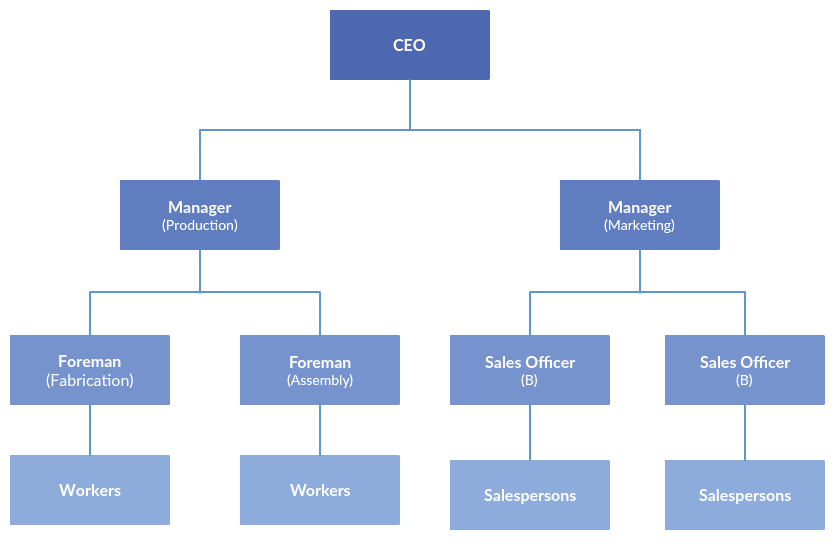
\includegraphics[scale=0.4]{gambar/organization-structure.png}
  % Keterangan gambar yang diinputkan
  \caption{Struktur organisasi PT. NASA}
  % Label referensi dari gambar yang diinputkan
  \label{fig:OrganizationStructure}
\end{figure}

% Contoh penggunaan referensi dari gambar yang diinputkan
Seperti yang bisa dilihat pada Gambar \ref{fig:OrganizationStructure}, \lipsum[15]
